\documentclass{book}
 
%Russian-specific packages
%--------------------------------------
\usepackage[T2A]{fontenc}
\usepackage[utf8]{inputenc}
\usepackage[russian,english]{babel}
\usepackage{amsmath}
\usepackage{amssymb}
%--------------------------------------
 
%Hyphenation rules
%--------------------------------------
%\usepackage{hyphenat}
%\hyphenation{ма-те-ма-ти-ка вос-ста-нав-ли-вать доп-пель-ган-гер гене-тика обще-научном}
%--------------------------------------
 
\usepackage{graphicx}
\begin{document}
\selectlanguage{russian}
%\tableofcontents

\chapter[Что такое не везёт: p-values]{Что такое не везёт и как это рассчитывать: p-values}

\section*{Cтатистическая значимость}

Словосочетание <<статистическая значимость>> (или его психологического доппельгангера, <<достоверность>>), наверное, слышали все. Медицина, генетика, опросы про зубную пасту и против зубной пасты - весь этот поток информации без статистики и без сравнения гипотез (вот для чего нужна значимость) превращается в хаос гигантских наборов данных.

Слово <<статистика>> имеет несколько значений. К более техническому, важному для нас, мы вернёмся позже, а сейчас поговорим немного об общенаучном. Статистика и теория вероятности - это связанные способы исследования закономерностей мира. Теория вероятностей предсказывает события, исходя из моделей, и так пытается понять то, что мы видим вокруг. Монетка, игральная кость, нормальное распределение - всё это модели случайных переменных, а исходы этих переменных - это те события, которые мы можем увидеть - орёл, четыре, лист длиной 4 сантиметра. Статистика же делает для теории вероятности черновую, обратную работу. Чтобы модель заработала, нужно знать её параметры, и статистика и занимается тем, что по многим наблюдениям делает утверждения о параметрах модели. Иногда эти утверждения - это оценки параметров модели (мы много говорили об этом в предыдущей главе), а иногда - и мы сейчас будем говорить об этом случае - это заключения о пригодности модели для описания наблюдений.

Семейство моделей, о которых мы говорим (вернее, с пониманием молчим), когда заходит речь о статистическая значимости или о p-value -- это модели, соответствующие нулевой гипотезе (Null Hypothesis). Конкретное содержание нулевой гипотезы зависит от предмета наблюдения, но общий смысл всегда один и тот же - всё плохо. Эта оптимистичная мысль объединяет собой все нулевые гипотезы. Лекарство работает так же, как плацебо, преступность не отличается между двумя городами, ген одинаково экспрессируется в разных условия, носители разных аллелей одного локуса одинаково часто болеют офигением -- всё это примеры нулевых гипотез. Если нулевая гипотеза верна, то в эксперименте, мы, конечно, всё равно не получим идеального сходства условий, идеального нуля в разности экспрессии генов и т.д. -- мы получим результат, порождённый шумом. Если же нулевая гипотеза не верна, то мы будем наблюдать некий содержательный сигнал, опять-таки искажённый шумом. Для того, чтобы на основании наблюдения (наблюдений), понять, насколько близка к истине нулевая гипотеза $\text{NULL}$ по сравнению с альтернативной (ненулевой) $\text{!NULL}$, используем формулы условной вероятности (теорему Байеса). 

\begin{align}\label{hyp_compare_bayes_null}
   &P\left(\text{NULL|obs}\right)=
   \frac{P\left(\text{obs|NULL}\right) P\left(\text{NULL}\right)}{P\left(\text{obs}\right)} = \nonumber \\
   &=\frac{P\left(\text{obs|NULL}\right) P\left(\text{NULL}\right)}{P\left(\text{obs|NULL}\right) P\left(\text{NULL}\right)+P\left(\text{obs|!NULL}\right) P\left(\text{!NULL}\right)} 
\end{align}
\begin{align}\label{hyp_compare_bayes_not_null}
   &P\left(\text{!NULL|obs}\right)=
   \frac{P\left(\text{obs|!NULL}\right) P\left(\text{!NULL}\right)}{P\left(\text{obs}\right)} = \nonumber \\
   &=\frac{P\left(\text{obs|!NULL}\right) P\left(\text{!NULL}\right)}{P\left(\text{obs|NULL}\right) P\left(\text{NULL}\right)+P\left(\text{obs|!NULL}\right) P\left(\text{!NULL}\right)}
\end{align}

При сравнении гипотез сокращают вероятность наблюдения $P\left(\text{obs}\right)$ (в англоязычной литературе она называется evidence), представленную одинаковой статсуммой в знаменателях \eqref{hyp_compare_bayes_null} и \eqref{hyp_compare_bayes_not_null} 

\begin{align}\label{hyp_compare_bayes_comp}
   &\frac{P\left(\text{NULL|obs}\right)}{P\left(\text{!NULL|obs}\right)}=\frac{P\left(\text{obs|NULL}\right) P\left(\text{NULL}\right)}{P\left(\text{obs|!NULL}\right) P\left(\text{!NULL}\right)}
\end{align}

Правильные и красивые формулы \eqref{hyp_compare_bayes_null}, \eqref{hyp_compare_bayes_not_null} и \eqref{hyp_compare_bayes_comp} на деле применяют редко: для них нужно уметь оценивать распределение экспериментальных результатов не только для нулевой гипотезы, но и для альтернативной, а это требует, как минимум, построения модели содержательного сигнала. 

\begin{figure}
    \centering
    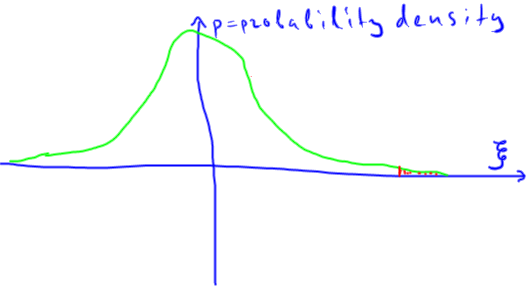
\includegraphics[scale=.5]{img/p-value.png}
    \caption{Площадь красного сегмента графика плотности вероятности случайной величины $\xi$ - это p-value, соответствующее значению $\xi$ на границе сегмента}
    \label{pval}
\end{figure}



 
\end{document}
